\documentclass[10pt,twocolumn,letterpaper]{article}

\usepackage{times}
\usepackage{epsfig}
\usepackage{graphicx}
\usepackage{amsmath}
\usepackage{amssymb}

\usepackage[a4paper, total={6.5in, 10in}]{geometry}

\usepackage[pagebackref=true,breaklinks=true,letterpaper=true,colorlinks,bookmarks=false]{hyperref}

\def\httilde{\mbox{\tt\raisebox{-.5ex}{\symbol{126}}}}


\begin{document}

\title{CSC320 Project}

\author{Jiatao Xiang\\
1004236613\\
{\tt\small jiatao.xiang@mail.utoronto.ca}
\and
Huakun Shen\\
{\tt\small huakun.shen@mail.utoronto.ca}
}

\maketitle


\section{Introduction}
Edge detection is a important tool in many computer vision applications. The major process of finding edge is to recognize sharp discontinuities in an image and mark them white whereas other places are marked black. Canny edge detection is one of the most famous algorithms that was invented by John Canny in 1986. And in this report, we will focus on how to improve Canny edge detection by modifying some steps of the algorithm.\\


\section{Background Information}
Canny Edge detection is a simple algorithm that is only consist of 5 steps. The first step is applying Gaussian filter. This is a pre-process step that can smooth out some noisy points in the image. The second step is to use Sobel filter (Gradient based filter) to extract the major edge of the image. The edge could be pretty wide. Non-maximum suppression is the third step of the algorithm. This step can thinning the wide edge, and make them one pixel wide. Next, the algorithm use threshold to separate the edges into 3 sections. They are strong pixels, weak pixels and zero pixels respectively. The final step (tracking process) is to track the weak pixels. The algorithm will keep all weak pixels that are connected to strong pixels and discard the others and assign them with zero intensity. The thinning process and tracking process provide precise edges in the result. This algorithm can also detect the edges in noisy state by applying the threshold methods.

\section{Proposal}
We gain a lot benefit from the Canny edge detection algorithm. However, there are also some drawbacks. We've list our concerns and possible improvements in the subsections below.

\subsection{Our concerns to the algorithm}
\begin{enumerate}
	\item[1.] In the first step, we have to choose patch size and sigma for Gaussian filter to get rid of the noisy points. If the value we choose is not property, the result will be unwilling.
	\item[2.] In the threshold step, the algorithm only have one high and low thresholds for the whole image, which may miss some detail that should be the edge or highlight something we do not want.
	\item[3.] The algorithm require a lot of computational time, which make the efficiency low.
\end{enumerate}

\subsection{Possible improvements}
\begin{enumerate}
	\item[1.] In stead of using Gaussian filter with user given patch size and sigma, we plan to use Gaussian pyramid instead (using reduce function when pre-process the image, and expand them back when we get the edge).
	\item[2.] We plan to identify multiple high and low thresholds by dividing image into different patches. For each patch, we calculate thresholds based on the highest intensity of pixel in that patch.
	\item[3.] Using reduce function multiple times to extract only the main features and after we get the edge image, we use expand function the same number of times to make the edge image the same size as the original image.
\end{enumerate}

\subsection{Reason for each improvements}
\begin{enumerate}
	\item[1.] Using Gaussian pyramid, we extract the main features of the image to reduce the noise. And the modified algorithm do not require user to give parameters for the Gaussian filter.
	\item[2.] We divide image into different patches and set different thresholds for each patch. In this way, we can extract main features for each patch, and in this way, the algorithm will reveal the edges that are omitted by original algorithm. 
	\item[3.] Using reduce function multiple times will reduce the size of image by a lot, which significantly improves the efficiency.
\end{enumerate}

\section{Gaussian Pyramid Experiment}
\subsection{Experiment setting}
Using Gaussian pyramid reduce function in the first step instead of Gaussian filter. Comparing the edges detected from original algorithm and modified algorithm on images with different noise level and the running time of the two algorithms.
\subsection{algorithm results}
\textbf{Set1:}\\
Parameters setting:\\
thresholds: [0.1, 0.3] for both algorithms\\
patch size: 3, sigma: 1 for original cannyEdge algorithm.\\
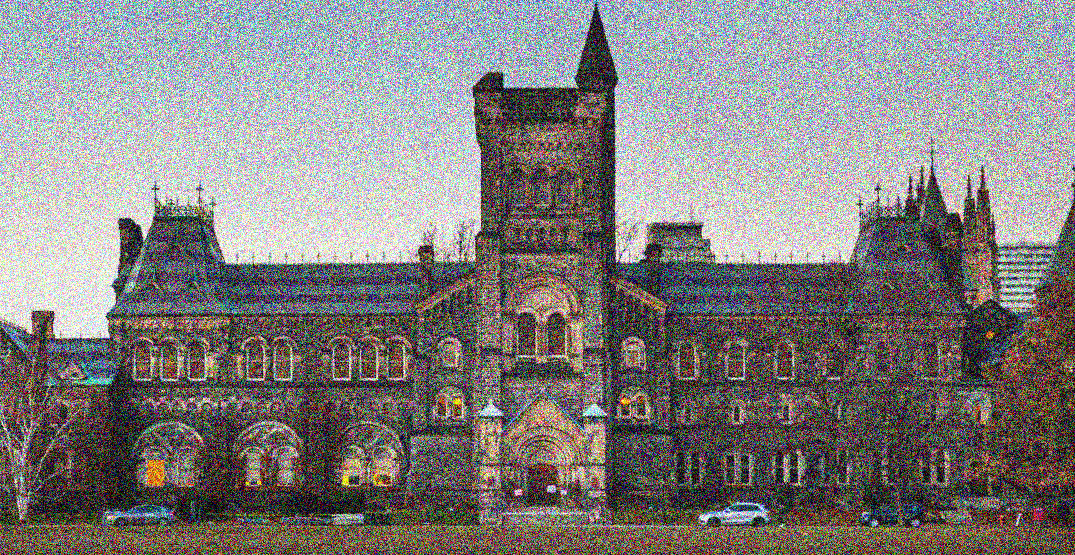
\includegraphics[scale=0.1]{UofT-noise-40.png}
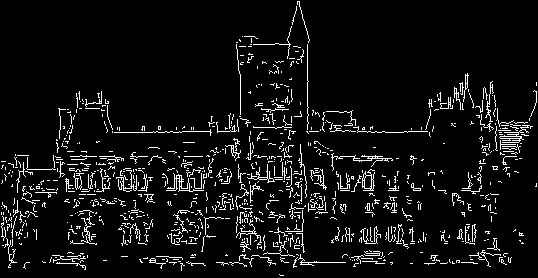
\includegraphics[scale=0.2]{pyramid_edge_noise_40.png}\\
original figure \hspace{45pt} modified algorithm result\\
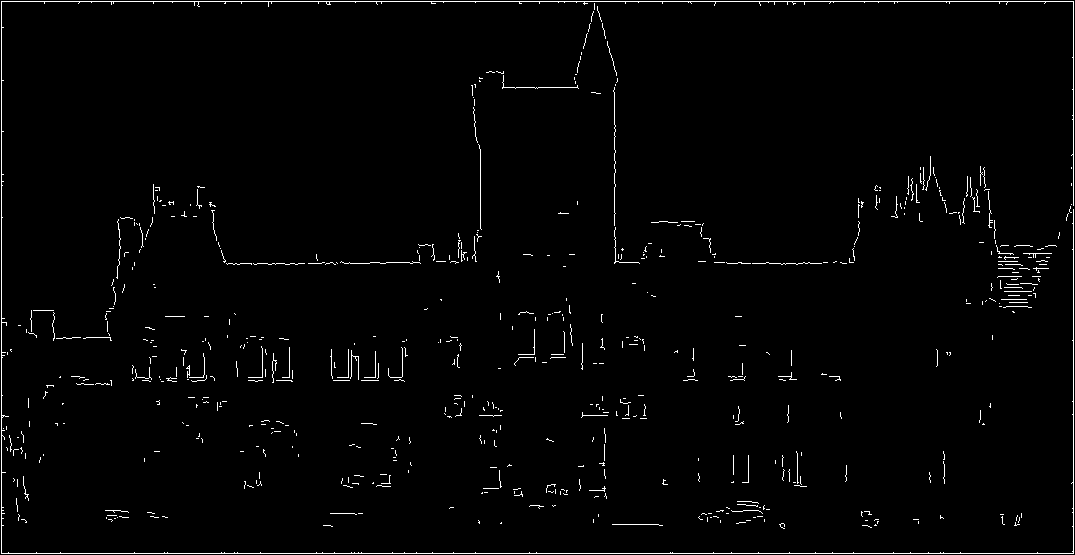
\includegraphics[scale=0.1]{result_original_noise_40.png}\\
original algorithm result\\
\\
\textbf{Set2:}\\
Parameters setting:\\
thresholds: [0.1, 0.3] for both algorithms\\
patch size: 3, sigma: 1 for original cannyEdge algorithm.\\
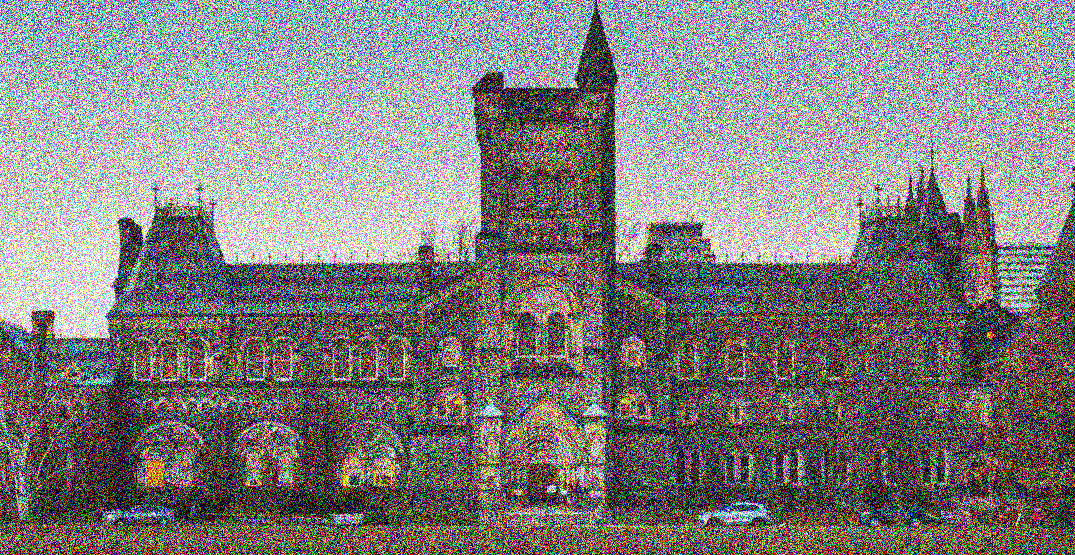
\includegraphics[scale=0.1]{UofT-noise-60.png}
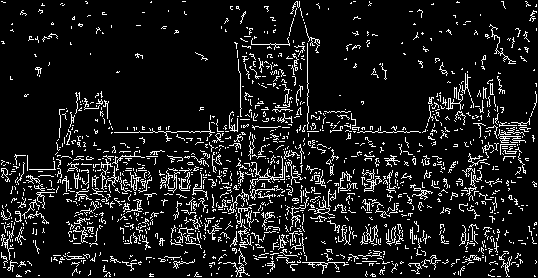
\includegraphics[scale=0.2]{pyramid_edge_noise_60.png}\\
original figure \hspace{45pt} modified algorithm result\\
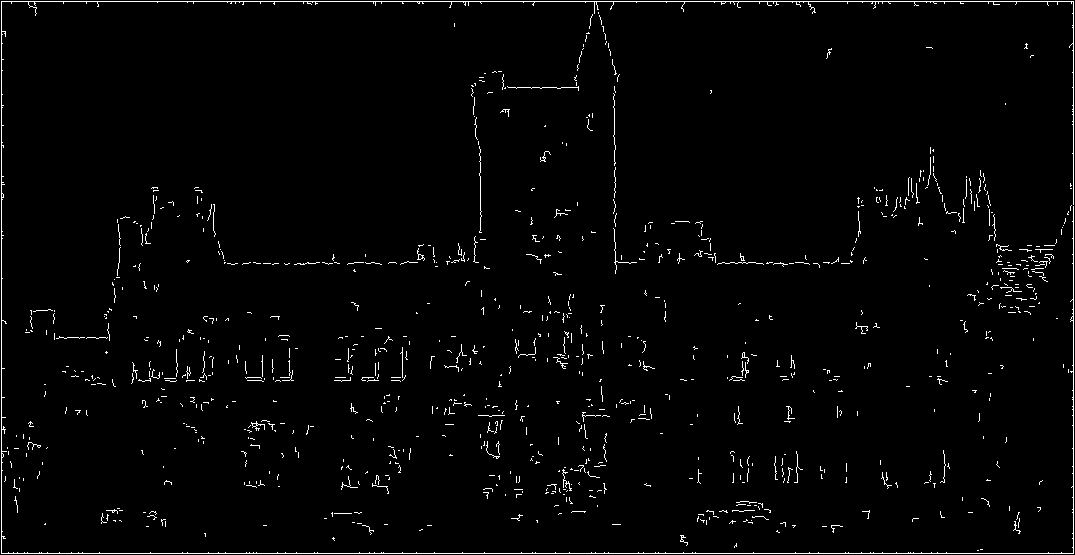
\includegraphics[scale=0.1]{result_original_noise_60.png}\\
original algorithm result\\
\\
\textbf{Set3:}\\
Same noise level as Set2\\
Parameters setting:\\
thresholds: [0.1, 0.4] for both algorithms\\
patch size: 3, sigma: 1 for original cannyEdge algorithm.\\
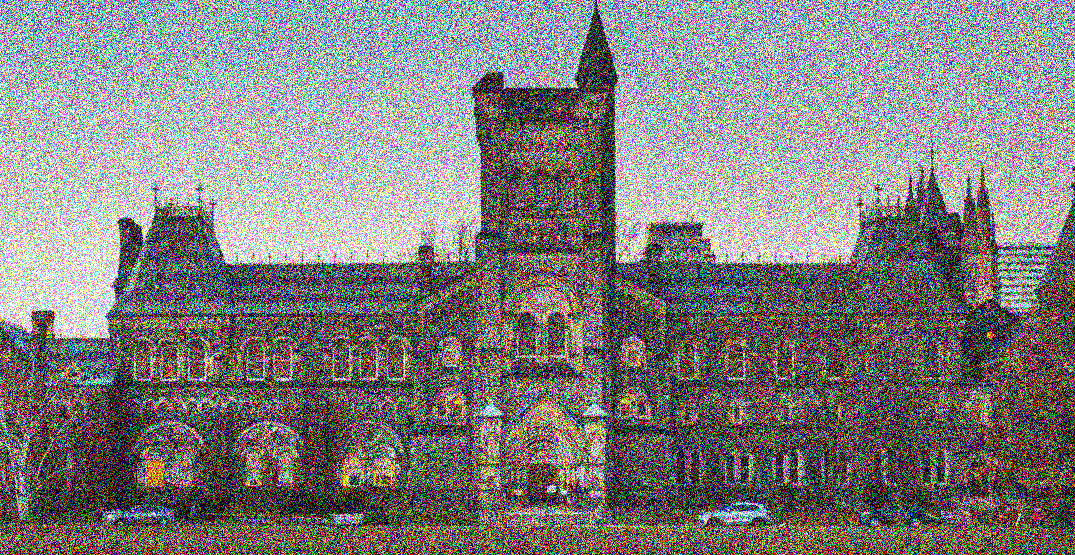
\includegraphics[scale=0.1]{UofT-noise-60.png}
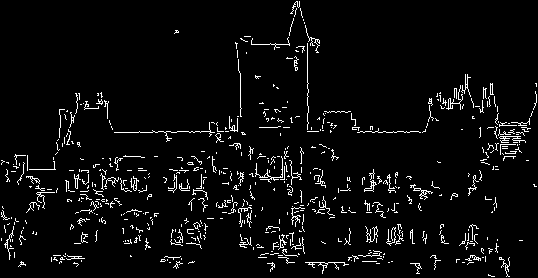
\includegraphics[scale=0.2]{pyramid_edge_noise_60_3.png}\\
original figure \hspace{45pt} modified algorithm result\\
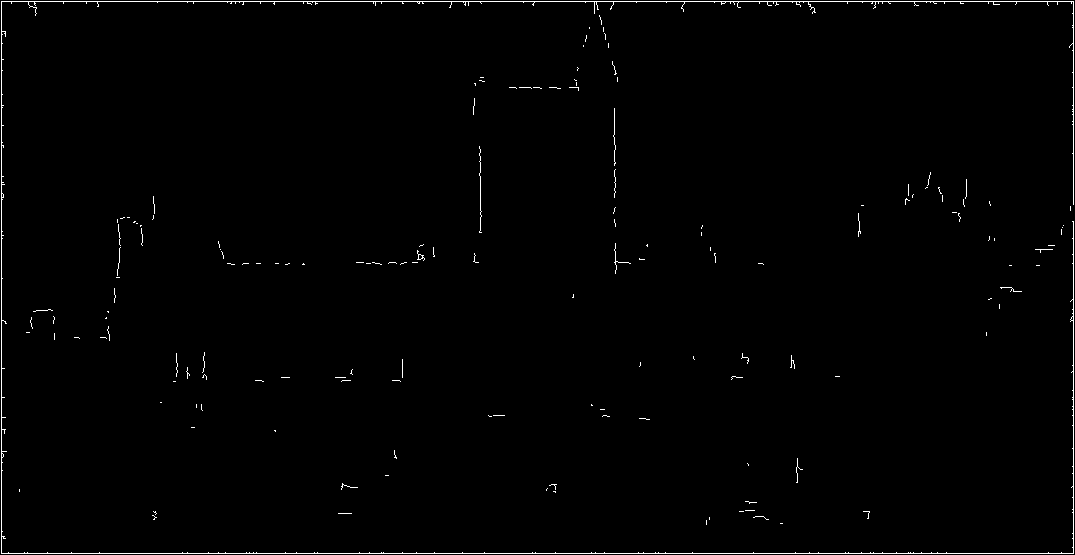
\includegraphics[scale=0.1]{result_original_noise_60_3.png}\\
original algorithm result\\
\\
\subsection{algorithm analysis}
\textbf{Set1:}\\
As we can see from the results of set1, the edge detected by modify algorithm captures more details, whereas the original algorithm only captures the outline of the building. This reveals that Gaussian filter could make some edges weak, so that those edges could not be detected by the algorithm. However, by using Gaussian pyramid reduce function, it extracts the main features from the original image and only smooth out the image by a little. This shows that if the user cannot find proper values for the parameters, our algorithm could outperform original algorithm because it doesn't affect the input image by a lot. Furthermore, finding good parameters are really time consuming because the domain of the parameters are in real number. This demonstrates that our algorithm is also better in the sense of user-friendly.\\
\\
\textbf{Set2:}\\
For the second experiment, we add more noise points to the input image. From the results, we can see that the modified algorithm thinks the noisy points are also the edges due to the sharp change in intensity. However, the result of the original algorithm is pretty clear and clean, which means the original algorithm could perform well even if the images are really noisy. It doesn't mean that the modified algorithm performs bad on noisy images because how this algorithm perform also depends on the high and low thresholds that we set.\\
\\
\textbf{Set3:}\\
In this experiment, we increase the high threshold to 0.4 and the result of the modified algorithm looks pretty good. This implies that even if the noise level is pretty high, we can modify threshold in order to make algorithm perform well. However, with this new threshold, the original algorithm cannot even captures the outline of the building. This experiment indicates the modified algorithm require higher high thresholds and the original algorithm require lower high thresholds. The good thing for modified algorithm is that it can captures the edge with more details, whereas for the original algorithm, it might lose those details due to the blur effect. 
\subsection{Conclusion}
\begin{enumerate}
	\item[1.] Modified algorithm is more user-friendly because it doesn't require user to give patch size and sigma, which is not easy to find.
	\item[2.] Modified algorithm could obtain edge with more details.
	\item[3.] Modified algorithm could also perform well on the images with high noise level if the thresholds are chosen properly.
	\item[4.] The running time of the modified algorithm is 4 times faster than the original one because it make the image size 1/4 of the original image.
\end{enumerate}
\subsection{limitation}
\begin{enumerate}
	\item[1.] The edge image found by modified algorithm is only 1/4 of the original one. Even if we use Gaussian pyramid expand function to reconstruct the result, the edge is blurred.
	\item[2.] The modified algorithm may perform bad if the image have a lot of sharp changes in intensity. 
\end{enumerate}

\section{Reference}
\end{document}
